\documentclass[conference]{IEEEtran}
\IEEEoverridecommandlockouts
% The preceding line is only needed to identify funding in the first footnote. If that is unneeded, please comment it out.
\usepackage{cite}
\usepackage{amsmath,amssymb,amsfonts}
\usepackage{graphicx}
\usepackage{textcomp}
\usepackage{xcolor}
\usepackage{fancyvrb}
\usepackage{listings}
\usepackage{hyperref}

\lstset{basicstyle=\scriptsize\ttfamily,breaklines=true}

\def\BibTeX{{\rm B\kern-.05em{\sc i\kern-.025em b}\kern-.08em
    T\kern-.1667em\lower.7ex\hbox{E}\kern-.125emX}}
\begin{document}

\title{Application of BagIt-Serialized Research Object Bundles for Packaging and Re-execution of Computational Analyses}

\author{

\IEEEauthorblockN{Kyle Chard}
\IEEEauthorblockA{\small{Computation Institute} \\
University of Chicago\\
Chicago, IL \\
chard@uchicago.edu}\\

\IEEEauthorblockN{Niall Gaffney}
\IEEEauthorblockA{\small{Texas Advanced Computing Center} \\
University of Texas at Austin\\
Austin, TX \\
ngaffney@tacc.utexas.edu}\\

\IEEEauthorblockN{Matthew B. Jones}
\IEEEauthorblockA{\small{NCEAS} \\
\small{University of California at Santa Barbara}\\
Santa Barbara, CA\\
jones@nceas.ucsb.edu}\\

\IEEEauthorblockN{Kacper Kowalik}
\IEEEauthorblockA{\small{NCSA} \\
\small{University of Illinois at Urbana-Champaign}\\
Champaign, IL\\
kowalikk@illinois.edu}\\

\and

\IEEEauthorblockN{Bertram Ludaescher}
\IEEEauthorblockA{\small{School of Information Sciences} \\
\small{University of Illinois at Urbana-Champaign}\\
Champaign, IL \\
ludaesch@illinois.edu}\\

\IEEEauthorblockN{Jarek Nabrzyski}
\IEEEauthorblockA{\small{Center for Research Computing} \\
\small{University of Notre Dame}\\
South Bend, IN\\
jaroslaw.nabrzyski.1@nd.edu}\\

\IEEEauthorblockN{Victoria Stodden}
\IEEEauthorblockA{\small{School of Information Sciences} \\
\small{University of Illinois at Urbana-Champaign}\\
Champaign, IL \\
vcs@stodden.net} \\

\IEEEauthorblockN{Ian Taylor}
\IEEEauthorblockA{\small{Center for Research Computing} \\
\small{University of Notre Dame}\\
South Bend, IN\\
ian.j.taylor@gmail.com} \\

\and

\IEEEauthorblockN{Thomas Thelen}
\IEEEauthorblockA{\small{NCEAS} \\
\small{University of California at Santa Barbara}\\
Santa Barbara, CA\\
thelen@nceas.ucsb.edu} \\

\IEEEauthorblockN{Matthew J. Turk}
\IEEEauthorblockA{\small{School of Information Sciences} \\
\small{University of Illinois at Urbana-Champaign}\\
Champaign, IL \\
mjturk@illinois.edu} \\

\IEEEauthorblockN{Craig Willis\IEEEauthorrefmark{2}}
\IEEEauthorblockA{\small{NCSA} \\
\small{University of Illinois at Urbana-Champaign}\\
Champaign, IL\\
willis8@illinois.edu}\\ 
\IEEEauthorrefmark{2}\footnotesize{\emph{Corresponding author}}
}



\maketitle

\begin{abstract}
In this paper we describe our experience adopting the Research Object Bundle format with BagIt 
serialization (BagIt-RO) for the design and implementation of tales in the NSF funded Whole Tale 
Project. A tale is an executable research object intended for the dissemination and publication of 
computational scientific findings that captures information needed to facilitate understanding, 
transparency, and re-execution for review and reproducibility at the time of publication. We 
describe the Whole Tale platform and requirements that led to our adoption of BagIt-RO, specifics 
of our implementation, and discuss migrating to the emerging Research Object Crate (RO-Crate) 
standard.
\end{abstract}

\begin{IEEEkeywords}
TBD
\end{IEEEkeywords}

\section{Introduction}


\cite{chard2016, chard2019, mecum2018, gentleman2007, brinckman2019}

Whole Tale (http://wholetale.org) is a web-based, open-source platform for reproducible research 
supporting the creation, sharing, execution, and verification of "tales." Tales are executable 
research objects that capture the code, data, and environment along with narrative and workflow 
information needed to re-create computational results from scientific studies. A goal of the Whole 
Tale platform is to produce an archival package that is exportable, publishable, and can be used 
for verification of computational reproducibility, for example as part of the peer-review process.

Since its inception, the Whole Tale platform has been designed to bring together existing open 
science infrastructure.  Researchers can ingest existing data from various scientific archival 
repositories; launch popular computational tools (e.g., Jupyter and RStudio); create and customize 
computational environments (using repo2docker); conduct analyses; create/upload code and data; and 
publish the resulting packages back to archival repositories. Tales are also downloadable and re-
executable locally, including support to retrieve remotely published data.  

With version 0.7 of the platform we adopted the Research Object Bundle BagIt serialization (BagIt-
RO) format. By combining the BagIt-RO serialization with our repo2docker-based execution framework 
and the BDBag tools \cite{chard2016}, we were able to  define and implement a standards-compliant, self-describing, portable, re-executable research object with the ability to retrieve remotely published data.

TODO:
[NEED SOME INTRO TO THE PAPER (e.g., mention that we first present a motivating example) then 
describe X, Y, Z.]


\section{Example scenario: Seal migration analysis}
The following scenario and Figure 1 illustrate the end-to-end Whole Tale workflow for exporting 
and publishing a tale based on existing data archived using the Research Workspace, a DataONE 
member node. This example is based on \cite{london2018, cameron2018}.

\emph{A research team is preparing to publish a manuscript describing a computational model for 
estimating animal movement paths from telemetry data.  The source data for their analysis, 
tracking data for juvenile seals in Alaska, has been published via the DataONE network. Using the 
Whole Tale platform, the researchers register the external dataset. They then create a new "tale" 
by launching an RStudio environment (based on the Rocker Project rocker/geospatial Docker image). 
Using the interactive environment, they clone a Github repository, modify an R Markdown document, 
customize the environment by specifying OS and R packages via repo2docker configuration files, and 
execute their code to generate outputs. Once they have verified their results, they enter 
descriptive metadata for the tale and publish the complete package back to DataONE to obtain a 
persistent identifier to include in publication. The researchers can optionally download the 
package in a compressed BagIt-RO format and run locally or share with others.}

\begin{figure}
\centering
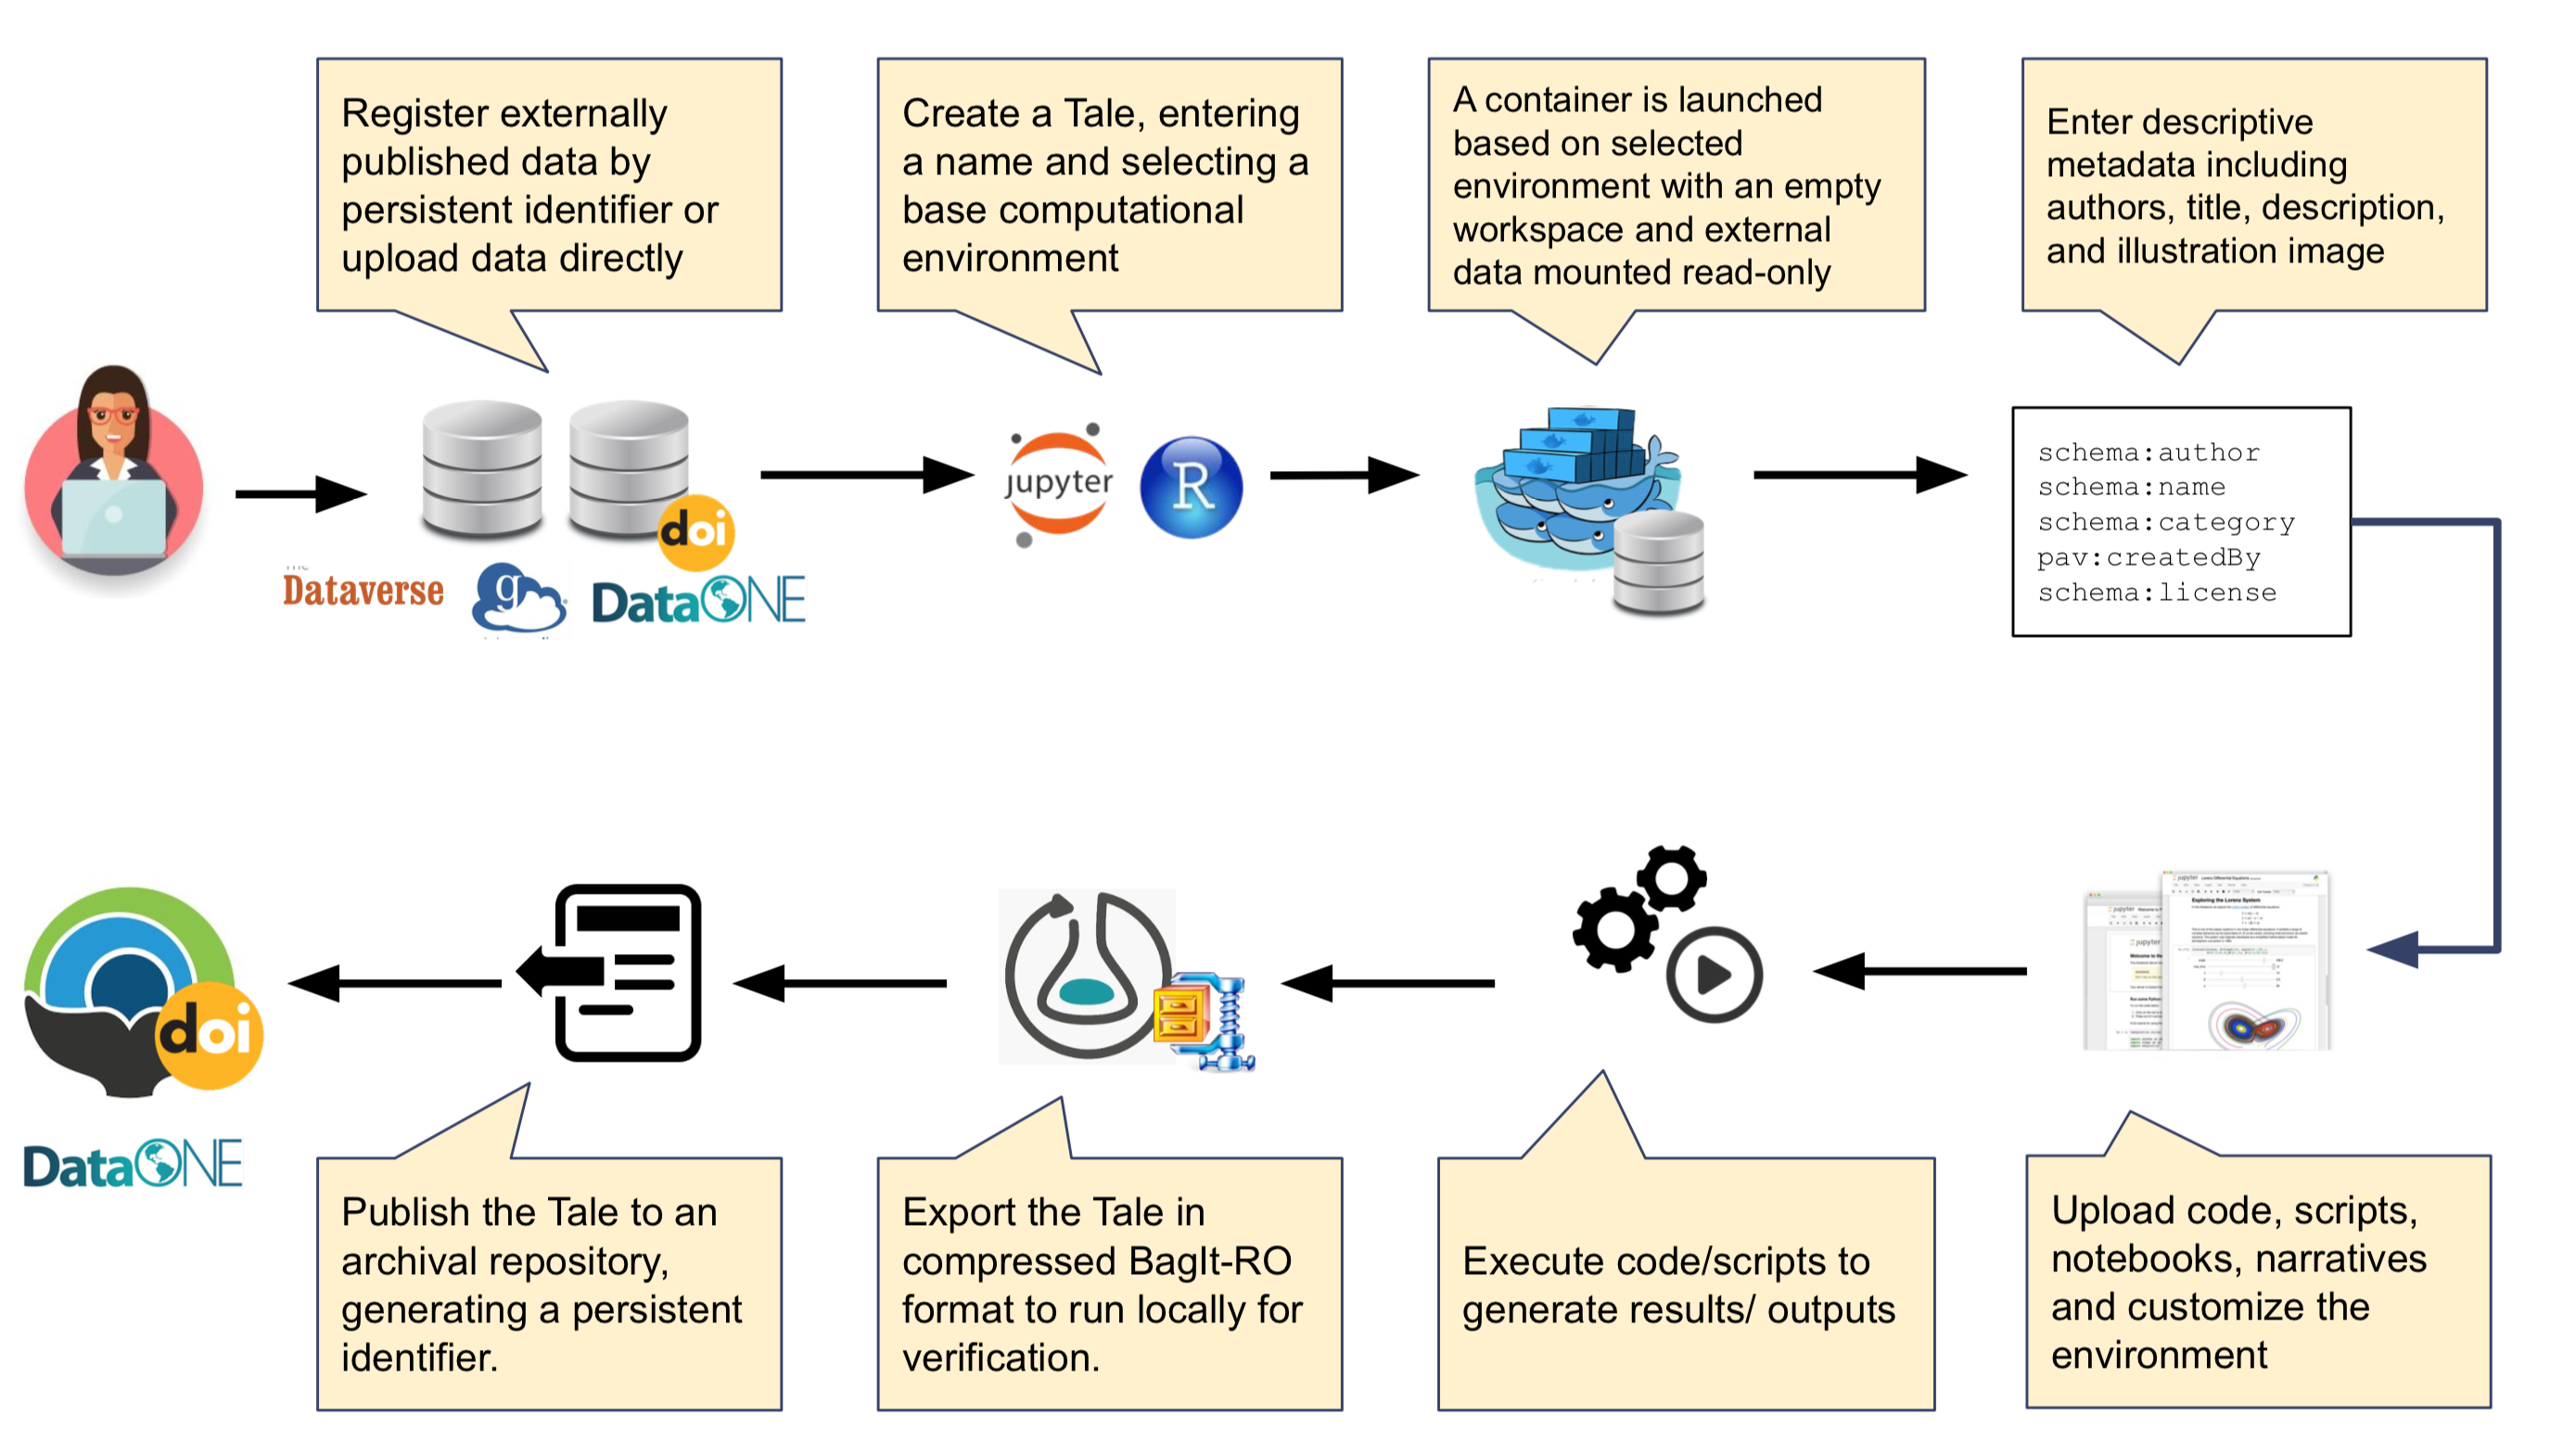
\includegraphics[scale=0.18]{images/wholetale-workflow.png}
\caption{Prototypical Whole Tale workflow}
\end{figure}


\section{System architecture}
This section provides a brief overview of the Whole Tale system architecture.   Whole Tale 
provides a scalable platform based on the Docker Swarm container orchestration system, exposing a 
set of core services via REST API and Single Page Application (SPA). Key components include:

\begin{figure}
\centering
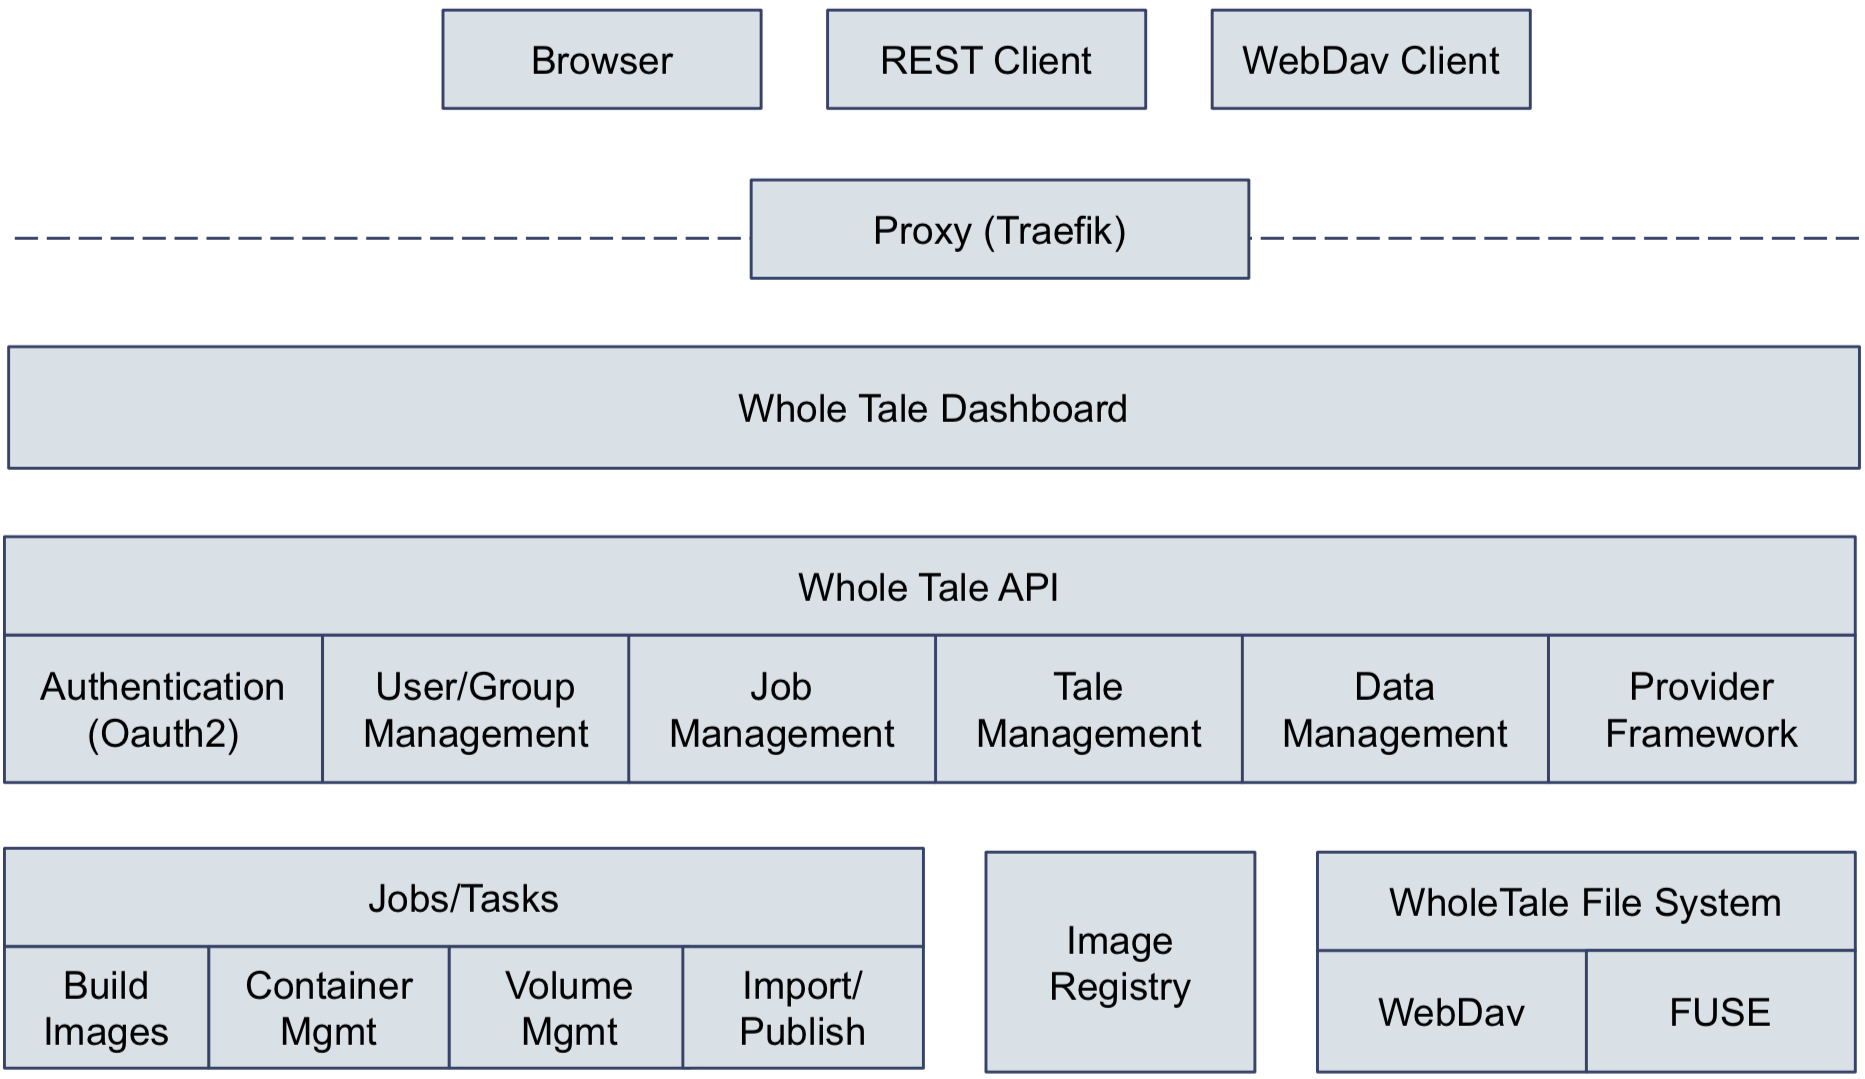
\includegraphics[scale=0.25]{images/wholetale-architecture.png}
\caption{Whole Tale system architecture}
\end{figure}

\begin{itemize}
\item{{\bf Whole Tale Dashboard}: Ember.js-based single page application}
\item{{\bf Whole Tale API}: REST API built using the Girder framework to expose key features including authentication, user/group management, tale creation lifecycle, data management, and integration with remote repositories ("providers")}
\item{{\bf Whole Tale File System}: A custom filesystem based on WebDav and FUSE used to mount user and registered data into running container environments}
\item{{\bf Image registry}: A local Docker registry to host images associated with tales}
\item{{\bf Job/tasks Management}: Task distribution and notification framework based on Girder and Celery Data Management System: System for fetching, caching, and exposing externally published datasets}
\end{itemize}

With respect to the BagIt-RO serialization format, the Whole Tale platform includes the following features:
\begin{itemize}
\item{User-defined tale environments that can be customized using an extension to the Binder project repo2docker component.}
\item{Tales can be exported in a BagIt-RO serialized archive that contains the contents of the tale workspace (code, local data, narrative, workflow, repo2docker configuration files) as well as references to external data, tale metadata, and script to run locally.}
\item{BDBag \cite{chard2016} can be used to materialize ?holey? bags by downloading files specified in the fetch.txt file , initially via HTTP and eventually via DOI, Globus, Agave schemes.}
\end{itemize}


\section{Requirements}
The scenario described above highlights several key requirements of the Whole Tale platform that 
led to our selection of the BagIt-RO serialization.  These requirements include:

\begin{itemize}
\item{{\bf Interoperability with archival repositories}: Since tales will be published to archival repositories including DataONE network members, we must adopt standard formats and vocabularies that facilitate interoperability. This includes the use of supported archival formats and identifiers (e.g., digital object identifiers). We also note here that some repositories do not support publishing hierarchical file structures, while many research objects contain data and code organized in folders. In the future, we plan to support publishing to Dataverse network members, the Dryad repository, and Zenodo.}
\item{{\bf Interoperability with source code management (SCM)}: For many researchers, source code repositories such as Github are central to their workflow in the creation of research objects. The tale format must support publishing research objects based on content in SCM repositories.}
\item{{\bf Ability to reference external data}: A central feature of the WT platform is to enable researchers to reference externally published data by persistent identifier and include references to those items in their published tales. Both in the WT web service and when executed locally, externally referenced data must be resolved prior to re-execution. Whole Tale currently supports HTTP resources as well as those published via Globus and in the future via the Agave Platform.}
\item{{\bf Ability to add metadata}: The Tale format must support all metadata attributes required by DataCite and schema.org as well as attributes specific to the WT platform. In the future, we expect to also support additional metadata required by researchers in specific domains.}
\item{{\bf Simplicity and understandability}: When users view the contents of an exported or published Tale, they should be able to easily understand the contents.}
\item{{\bf Ability to export and re-execute}: One feature of the system is the ability for users to export Tales to a local machine. To re-run locally, we must be able to rebuild the environment (e.g., via Docker/repo2docker) and fetch remote data as needed.}
\item{{\bf Ability to store provenance information}: Future releases of WT, Tales will include computational and archival provenance information.}
\item{{\bf Verifiability}: Future releases of WT will include information to allow the automatic re-execution and verification of included computational workflows.}
\item{{\bf Versioning}: Since researchers iterate on their tales, share them and extend them, it is important to be able to version them over time.}
\item{{\bf Interoperability with search engines}: Google recently unveiled Dataset Search which parses and aggregates JSON-LD embedded on dataset landing pages as an effort to lower barriers for finding datasets. Choosing JSON-LD as a representation for Tale metadata provides flexibility in case we decide to expose Tale information for Google. It also allows for further integration with third party publishers such as Dataverse and DataONE who may expose such metadata for Google.}
\end{itemize}

\section{Example Tale}

In this section, we outline the contents of an exported tale. The complete example is available at https://doi.org/10.5281/zenodo.2641314.


\begin{center}
\begin{footnotesize}
\begin{tabular}{| p{4cm}|p{4cm} | } \hline
{\bf File} & {\bf Description}  \\ \hline
\texttt{bag-info.txt} & Bag metadata using the bdbag-ro-profile \\ \hline
\texttt{bagit.txt} & Bag declaration \\ \hline
\begin{minipage}{3in}
\begin{scriptsize}
\begin{verbatim}

data/
  LICENSE
  workspace/
    apt.txt
    postBuild
    requirements.txt
    wt_quickstart.ipynb
\end{verbatim}
\end{scriptsize}
\end{minipage} & Payload directory containing tale license and workspace including repo2docker compatible configuration files. \\ \hline
\texttt{fetch.txt} & Fetch file \\ \hline
\texttt{manifest-[md5, sha256].txt} & Payload manifest \\ \hline
\begin{minipage}{3in}
\begin{scriptsize}
\begin{verbatim}

metadata/
    manifest.json
    environment.json
\end{verbatim}
\end{scriptsize}
\end{minipage} &  Tag directory containing RO manifest.json and Whole Tale environment metadata  (required by repo2docker\_wholetale) \\ \hline
\texttt{tagmanifest-[md5, sha256].txt} & Tag manifest  \\ \hline
\texttt{README.md} & Tale top-level readme \\ \hline
\texttt{run-local.sh} & Tale local execution script \\ \hline
\end{tabular}
\end{footnotesize}
\end{center}






\section{Adopting the BagIt-RO Model}

Whole Tale uses the RDF data model to encode tale information for export and exchange. We selected 
a JSON-LD representation for human readability, extensibility, compatibility with Whole Tale APIs, 
and potential interoperability with search engines and third party publishers. After developing an 
ad-hoc internal format, we explored emerging standards in the research object space and settled on 
BagIt-RO for serialization. The RO-Bundle specification and BagIt serialization including 
compatibility with bdbag tools met many of our initial requirements.  Additional tale metadata 
attributes which were not included in the BagIt-RO model could be added using vocabularies such as 
schema.org and MADS.  Throughout this section, we use the manifest.json from the above example, 
included in Appendix A.

\subsection{Filesystem Artifacts}
One strong point of RO-Bundle is that it treats file system artifacts as aggregates of the 
manifest. Doing so satisfies our requirement of being able to track where files belong, enabling 
us to both export and re-import tales. In the case of Whole Tale, artifacts include data that were 
retrieved from external repositories as well as files that the user uploaded to the system from 
their local machine to the tale workspace. The tale workspace contents are included in the payload 
"data/workspace" directory and the external data are fetched into the payload "data/data" 
directory, mirroring filesystem organization on the web-based platform.

\begin{lstlisting}
  "aggregates": [
    {
      "uri": "../data/workspace/wt_quickstart.ipynb"
    },
    {
      "uri": "../data/workspace/apt.txt"
    }
  ]
\end{lstlisting}

Local system artifacts are easily described with a single URI entry. Some files, such as the 
system generated readme are tagged with additional metadata, shown below. In this case the 
additional metadata specifies the ?type? of the file as a ?HowTo? file.

\begin{lstlisting}
  {
    "@type": "HowTo",
    "uri": "../README.md"
  }
\end{lstlisting}

\subsection{External data}

Whole Tale supports two types of external data: data that resides in a repository identified by 
persistent identifier (e.g., DOI) and data that exists at a generic HTTP address. In addition to 
including information about external data in the manifest.json, regardless of type the URL for 
each remote file is included in the fetch.txt for retrieval using BDBag tools.

\subsubsection{Generic HTTP Data}
For data that doesn?t belong to a remote repository, a simple bundle is created in the aggregation section. The URI points to the HTTP address where the file may be retrieved and the bundle object holds the filesystem relevant information. The combination of information allows us to retrieve the file and place it in the correct folder (i.e., data/data).

\subsubsection{Repository Data}
Additional metadata can be compiled when files included from published datasets are brought into 
the system. The individual files are described with a single bundle object, and linked to an 
additional structure that describes the dataset in more detail.

The following snippet describes a remote dataset that resides in DataONE and the aggregation 
recording the relationship between a file in that dataset and its ultimate location after 
retrieval:


\begin{lstlisting}
 "dataset": [
   "@type": "Dataset",
   "identifier": "doi:10.5065/D6862DM8",
   "name": "Humans and Hydrology at High Latitudes...",
   "@id": "doi:10.5065/D6862DM8"
  ],
  "aggregates": [
    {
      "size": 1558016,
      "schema:isPartOf": "doi:10.5065/D6862DM8",
      "uri": "https://cn.dataone.org/cn/v2/resolve/urn:...",
      "bundledAs": {
          "filename": "usco2000.xls",
          "folder": "../data/data/"
      }
    }
]
\end{lstlisting}

\subsection{Describing the Computing Environment}
Whole Tale uses a customized version off the Binder repo2docker system. In addition to including 
configuration files in the workspace, Whole Tale exports information about the environment 
including runtime information in the exported package. One shortcoming of the BagIt-RO model is 
that there is not a well-defined place for this metadata. To address this need, we define an 
additional tag file, environment.json, which encodes sufficient information about the environment 
so that it can be re-created. The metadata contained in this file is represented as JSON and is 
not described using standard vocabularies. 

\subsection{Describing Additional Attributes}
A number of properties that describe additional tale attributes (e.g., authors?) are defined at 
the manifest root. Schema.org?s vocabulary sufficed for describing these general metadata fields.

Attributing authorship to a Tale is a requirement for tracking researcher contributions and is 
also used during metadata generation with publishers. The pav vocabulary is used instead of schema 
because the BagIt-RO specification already uses it.

\begin{lstlisting}
   {
      "@id": "https://orcid.org/0000-0002-7523-5539",
      "@type": "schema:Person",
      "schema:familyName": "DeBruine",
      "schema:givenName": "Lisa"
    }
\end{lstlisting}
		
		
\subsection{Provenance Tracking}

A planned feature of Whole Tale is the ability to track executions and steps in researchers? 
workflows. The BagIt-RO model provides an easy way to represent this on disk with our proposed 
method through the inclusion of a provenance.json. One difference is that we plan to use the Prov-
ONE ontology, an extension to W3C PROV.

The URI of each file in the manifest can be referenced inside the provenance.json file, enabling 
rich linkings of information. This information can also be transcribed to publisher-specific 
formats, provided that they support PROV.

\begin{figure}
\centering
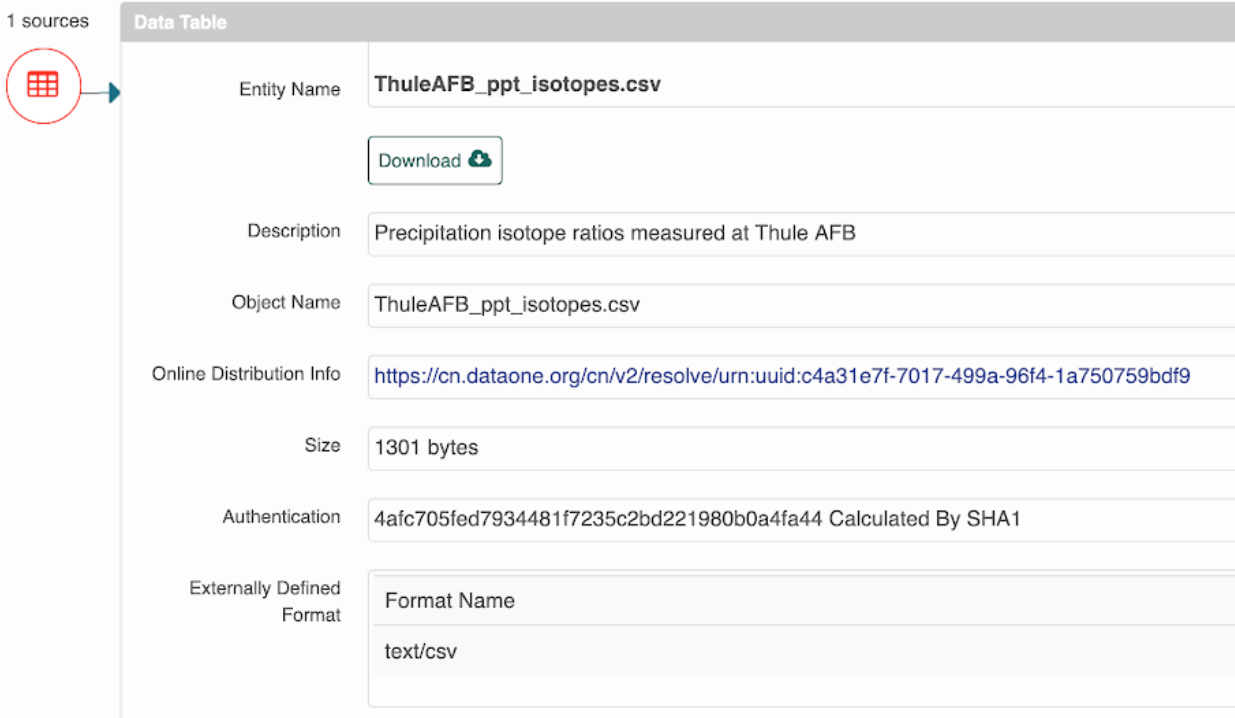
\includegraphics[scale=0.25]{images/dataone-prov.png}
\caption{Provenance rendering of a file in DataONE}
\end{figure}


\section{Discussion}

\subsection{Migrating to RO-Crate}
Since our adoption of the BagIt-RO model, the community has moved forward on the Research Object 
Crate (RO-Crate) specification. In this section, we report the results of a preliminary analysis 
of changes needed to migrate to the new format.  Doing so will require versioning the tale export 
format and will not make changes until the community settles on a near-final version of the 
specification.

RO-Crate 0.2-DRAFT introduces the following changes from the RO-Bundle 1.0
\begin{itemize}
\item{Addition of ro-crate-metadata.jsonld (RO-Crate Metadata File). The relationship to the RO-Bundle manifest.json is unclear, since the RO-Crate Metadata File "does not necessarily list or describe all files in the package." We have viewed the "manifest.json" as an inventory of all files in the RO (excluding those introduced by BagIt).}
\item{The RO-Crate metadata file changes vocabulary from the set used by RO-Bundle to primarily schema.org, no longer using ore:aggregates. This also adds support for referencing external datasets, a feature not available in RO-Bundle but added in our tale format.}
\item{The "bagged" RO-Crate structure will differ from the BagIt-RO structure as the "metadata" folder is no longer included.  Our assumption is that the ro-crate-metadata.jsonld along with our environment.json will now be included in the BagIt payload. We've come to a similar conclusion about the tale format -- that this metadata belongs in the payload not external to it.}
\item{It is unclear whether there will be support for separate provance metadata or whether this will need to be included in the payload.}
\end{itemize}

RO-Crate promises many benefits that align with Whole Tale, namely the adoption of schema.org as the primary vocabulary and its ability to be used alongside a variety of export formats. 


\subsection{BagIt Understandability}

One drawback of the BagIt serialization is that the BagIt configuration is foregrounded and 
difficult to understand for the average researcher/user while the "payload" directory is less 
apparent and confusingly named "data". Although out of scope for the RO discussion, we are 
supportive of the idea of a ".bagit" directory that contains the relevant configuration 
information.

\subsection{External data}
In the Whole Tale platform, users are presented with a fixed filesystem hierarchy that includes  
"workspace" and "data" directories. The workspace directory contains code, local data, and 
additional files (e.g., documentation) and the sibling "data" directory contains externally 
reference data files (read-only).

In our v0.7 release, the payload directory of an exported tale similarly contains "workspace" and 
"data" directories. The manifest.json contains information about remotely registered datasets that 
is also included in the BagIt fetch.txt.  When BDBag tools are used to fetch remote datasets, they 
are downloaded to the payload/data directory, matching the online filesystem organization and 
system capabilities.  The concept of the fetch.txt, while primitive, was surprisingly effective 
when used with BDBag. We also foresee taking advantage of other BDBag capabilities, such as 
transferring Globus data or using DOI protocol. However, there is redundancy in tracking external 
information in both in the BagIt fetch.txt and the RO manifest.json. While we originally 
considered serializing tales in multiple formats, settling on the BagIt-RO serialization provided 
significant convenience.

\subsection{Relationship to VCS}
For many researchers, a version control system repository maps to a particular research 
compendium/research object for publication. Researchers are increasingly using services such as 
GitHub for collaboration, tagging or releasing versions of their projects, and publishing them via 
external tools (e.g., Zenodo, Whole Tale).  In the Whole Tale platform, the "workspace" directory 
equates to (and can be mapped to) a version controlled  repository.  The question becomes whether 
or not the workspace or repository should contain everything, including the information in the 
manifest.json and environment.json.  During the local execution process, for technical reasons we 
bind mount files from the "metadata" directory into the workspace to support building the tale 
image.  In future releases, we are considering exposing the manifest information along with 
provenance information (below) as part of the workspace instead of external to it, such as in the 
RO-Bundle metadata directory.  This means that even simple metadata would be in the workspace and 
easily added to VCS.

\subsection{Provenance}
In the BagIt-RO examples and our thinking for v0.7, computational provenance information including 
that created by the user or by the Whole Tale platformwould be stored in the "metadata" directory 
alongside the manifest.  As with the discussion of VCS systems above, we question whether 
provenance information is external to or part of the RO itself.  Certainly some provenance 
information, such as archival provenance as the RO moves through a curation process, is external 
to the RO itself. But computational provenance related to the execution of the code within the RO 
seems to be a component of the RO and should be part of the payload.

\subsection{Executable Research Objects}
Tales are executable research objects. This means that the research object itself defines an 
environment that can be built and re-executed to possibly verify results. While this is not a 
unique capability (supported also by CodeOcean, Binder, etc), it is worth highlighting in this 
workshop as we consider other types of research objects.


\subsection{Verification}
Lacking a place for the compute environment info (environment.json isn?t JSON-LD) and isn?t directly supported by bd-bag


\subsection{Conclusions}
By implementing an extension to RO-Bundle with BagIt serialization and leveraging existing open science infrastructure tools including repo2docker and BDBag, we were able to effectively create an exportable, publishable, and executable research object package.  While not a perfect fit, BagIt-RO met many of our platform requirements. We expect to continue work in this area as we add support for computational provenance information and automated verification and hope to contribute to the use cases and discussions that inform the development of a broader community standard.

\section*{Acknowledgment}

The preferred spelling of the word ``acknowledgment'' in America is without 
an ``e'' after the ``g''. Avoid the stilted expression ``one of us (R. B. 
G.) thanks $\ldots$''. Instead, try ``R. B. G. thanks$\ldots$''. Put sponsor 
acknowledgments in the unnumbered footnote on the first page.

\section*{References}

\bibliographystyle{abbrv}
\bibliography{bibliography}

\section{Appendix A}
\begin{lstlisting}
{
    "createdBy": {
        "@type": "schema:Person",
        "schema:givenName": "Craig",
        "@id": "willis8@illinois.edu",
        "schema:email": "willis8@illinois.edu",
        "schema:familyName": "Willis"
    },
    "schema:description": "Demonstration of how to use Whole Tale to develop custom analysis and visualization for data published externally via DataONE.  See https://wholetale.readthedocs.io/en/stable/users_guide/quickstart.html for more information.",
    "@context": [
        "https://w3id.org/bundle/context",
        {
            "schema": "http://schema.org/"
        },
        {
            "Datasets": {
                "@type": "@id"
            }
        }
    ],
    "schema:author": [
        {
            "@type": "schema:Person",
            "schema:givenName": "Craig",
            "@id": "https://orcid.org/0000-0002-6148-7196",
            "schema:familyName": "Willis"
        }
    ],
    "schema:version": 7,
    "schema:identifier": "5cb4ffead9323600016c4d4c",
    "schema:image": "http://use.yt/upload/dc1da723",
    "Datasets": [
        {
            "@type": "Dataset",
            "identifier": "doi:10.5065/D6862DM8",
            "name": "Humans and Hydrology at High Latitudes: Water Use Information",
            "@id": "doi:10.5065/D6862DM8"
        }
    ],
    "createdOn": "2019-04-15 22:04:26.970000",
    "schema:name": "Example Water Tale",
    "schema:category": "Examples",
    "aggregates": [
        {
            "uri": "../data/workspace/wt_quickstart.ipynb"
        },
        {
            "uri": "../data/workspace/apt.txt"
        },
        {
            "uri": "../data/workspace/requirements.txt"
        },
        {
            "uri": "../data/workspace/postBuild"
        },
        {
            "size": 1558016,
            "schema:isPartOf": "doi:10.5065/D6862DM8",
            "uri": "https://cn.dataone.org/cn/v2/resolve/urn:uuid:62e1a8c5-406b-43f9-9234-1415277674cb",
            "bundledAs": {
                "filename": "usco2000.xls",
                "folder": "../data/data/"
            }
        },
        {
            "schema:license": "CC-BY-4.0",
            "uri": "../data/LICENSE"
        },
        {
            "@type": "schema:HowTo",
            "uri": "../data/README.md"
        }
    ],
    "@id": "https://data.wholetale.org/api/v1/tale/5cb4ffead9323600016c4d4c"
}
\end{verbatim}
\end{lstlisting}


\end{document}
